\documentclass{article}%
\usepackage[T1]{fontenc}%
\usepackage[utf8]{inputenc}%
\usepackage{lmodern}%
\usepackage{textcomp}%
\usepackage{lastpage}%
\usepackage{parskip}%
\usepackage[top=1.2in,bottom=1in,left=0.6in,right=0.6in,headsep=0.8in]{geometry}%
\usepackage{amsmath}%
\usepackage{graphicx}%
\usepackage{needspace}%
\usepackage{color}%
\usepackage{longtable}%
\usepackage{multirow}%
\usepackage[table]{xcolor}%
\usepackage{fancyhdr}%
\usepackage{tabularx}%
%
\definecolor{OsdagGreen}{HTML}{D5DF93}%
\fancypagestyle{header}{ 
\renewcommand{\headrulewidth}{0pt}%
\renewcommand{\footrulewidth}{0pt}%
\fancyhead{ 
}%
\fancyfoot{ 
}%
\fancyhead[C]{ 
\begin{tabularx}{\textwidth}{|l|p{6cm}|l|X|}%
\hline%
\rowcolor{OsdagGreen}%
Company Name&LoremIpsum&Project Title&Fossee\\%
\hline%
\rowcolor{OsdagGreen}%
Group/Team Name&LoremIpsum&Subtitle&\\%
\hline%
\rowcolor{OsdagGreen}%
Designer&LoremIpsum&Job Number&123\\%
\hline%
\rowcolor{OsdagGreen}%
Date&26 /05 /2020&Client&LoremIpsum\\%
\hline%
\end{tabularx}
}%
\fancyfoot[R]{ 
Page \thepage\ of \pageref{LastPage}
}
}%
%
\begin{document}%
\normalsize%
\pagestyle{header}%
\section{Input Parameters}%
\label{sec:InputParameters}%
\renewcommand{\arraystretch}{1.2}%
\begin{longtable}{|p{5cm}|p{2cm}|p{2cm}|p{2cm}|p{5cm}|}%
\hline%
\hline%
\multicolumn{3}{|c|}{Module}&\multicolumn{2}{|c|}{Beam Coverplate Weld Connection}\\%
\hline%
\hline%
\multicolumn{3}{|c|}{MainModule}&\multicolumn{2}{|c|}{Moment Connection}\\%
\hline%
\hline%
\multicolumn{3}{|c|}{Moment(kNm)*}&\multicolumn{2}{|c|}{10.0}\\%
\hline%
\hline%
\multicolumn{3}{|c|}{Shear (kN)*}&\multicolumn{2}{|c|}{100.0}\\%
\hline%
\hline%
\multicolumn{3}{|c|}{Axial (kN) *}&\multicolumn{2}{|c|}{80.0}\\%
\hline%
\hline%
\multicolumn{5}{|c|}{\textbf{Section}}\\%
\hline%
\hline%
\multirow{12}{*}{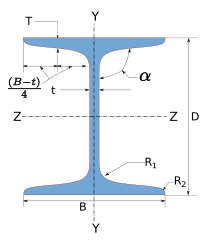
\includegraphics[width=5cm,height=5cm]{E:/office _anjali/columnspliceanjali/Osdag3/ResourceFiles/images/ISection.png}}&\multicolumn{2}{|c|}{Beam Section *}&\multicolumn{2}{|c|}{NPB 300x150x36.5}\\%
\cline{2%
-%
5}%
&\multicolumn{2}{|c|}{Preferences}&\multicolumn{2}{|c|}{Outside}\\%
\cline{2%
-%
5}%
&\multicolumn{2}{|c|}{Material *}&\multicolumn{2}{|c|}{E 250 (Fe 410 W)A}\\%
\cline{2%
-%
5}%
&\multicolumn{2}{|c|}{Ultimate strength, fu (MPa)}&\multicolumn{2}{|c|}{410}\\%
\cline{2%
-%
5}%
&Yield Strength , fy (MPa)&250&R1(mm)&1.5\\%
\cline{2%
-%
5}%
&Mass&36.52&R2(mm)&0.0\\%
\cline{2%
-%
5}%
&Area(mm2) {-} A&4650.0&Iz(mm4)&71735000.0\\%
\cline{2%
-%
5}%
&D(mm)&297.0&Iy(mm4)&5183900.0\\%
\cline{2%
-%
5}%
&B(mm)&150.0&rz(mm)&124.2\\%
\cline{2%
-%
5}%
&t(mm)&6.1&ry(mm)&33.4\\%
\cline{2%
-%
5}%
&T(mm)&9.2&Zz(mm3)&483060.0\\%
\cline{2%
-%
5}%
&FlangeSlope&90&Zy(mm3)&69120.0\\%
\cline{2%
-%
5}%
\hline%
\multicolumn{5}{|c|}{\textbf{Weld Details}}\\%
\hline%
\hline%
\multicolumn{3}{|c|}{Weld Type}&\multicolumn{2}{|c|}{Fillet}\\%
\hline%
\hline%
\multicolumn{3}{|c|}{Type of weld fabrication}&\multicolumn{2}{|c|}{Shop Weld}\\%
\hline%
\hline%
\multicolumn{3}{|c|}{Material grade overwrite (MPa) Fu}&\multicolumn{2}{|c|}{410.0}\\%
\hline%
\hline%
\multicolumn{5}{|c|}{\textbf{Safety Factors {-} IS 800:2007 Table 5 (Clause 5.4.1) }}\\%
\hline%
\hline%
\multicolumn{3}{|c|}{Governed by Yielding}&\multicolumn{2}{|c|}{$\begin{aligned}\gamma_{m0}&=1.1\end{aligned}$}\\%
\hline%
\hline%
\multicolumn{3}{|c|}{Governed by Ultimate Stress}&\multicolumn{2}{|c|}{$\begin{aligned}\gamma_{m1}&=1.25\end{aligned}$}\\%
\hline%
\hline%
\multicolumn{3}{|c|}{Connection Weld}&\multicolumn{2}{|c|}{$\begin{aligned}\gamma_{mw}&=1.25\end{aligned}$}\\%
\hline%
\end{longtable}

%
\Needspace{10\baselineskip}%
\newpage%
\section{Design Checks}%
\label{sec:DesignChecks}%
\subsection{Member Capacity}%
\label{subsec:MemberCapacity}%
\renewcommand{\arraystretch}{1.2}%
\begin{longtable}{|p{4cm}|p{5cm}|p{5.5cm}|p{1.5cm}|}%
\hline%
\rowcolor{OsdagGreen}%
Check&Required&Provided&Remarks\\%
\hline%
\endhead%
\hline%
Axial Capacity Member Ac (kN)&&$\begin{aligned} A_c &=\frac{A*f_y}{\gamma_{m0} *10^3}\\ &=\frac{4650.0*250}{1.1* 10^3}\\ &=1056.82\end{aligned}$&\\%
\hline%
Shear Capacity Member Sc (kN)&&$\begin{aligned} S_c &= \frac{A_v*f_y}{\sqrt{3}*\gamma_{mo} *10^3}\\ &=\frac{278.6*6.1*250}{\sqrt{3}*1.1 *10^3}\\ &=223.0\end{aligned}$&\\%
\hline%
Plastic Moment Capacity Pmc (kNm)&&$\begin{aligned} Pmc &= \frac{\beta_b * Z_p *fy}{\gamma_{mo} * 10^6}\\ &=\frac{1*118367.39*250}{1.1 * 10^6}\\ &=26.9\end{aligned}$&\\%
\hline%
Moment Deformation Criteria Mdc (kNm)&&$\begin{aligned} Mdc &= \frac{1.5 *Z_e *fy}{1.1* 10^6}\\ &= \frac{1.5 *483060.0*250}{1.1* 10^6}\\ &= 164.68\end{aligned}$&\\%
\hline%
Moment Capacity Member Mc (kNm)&&$\begin{aligned} M_c &= min(Pmc,Mdc)\\ &=min(26.9,164.68)\\ &=26.9\end{aligned}$&\\%
\hline%
\end{longtable}

%
\newpage%
\subsection{Load Consideration}%
\label{subsec:LoadConsideration}%
\renewcommand{\arraystretch}{1.2}%
\begin{longtable}{|p{4cm}|p{3.5cm}|p{6.5cm}|p{1.5cm}|}%
\hline%
\rowcolor{OsdagGreen}%
Check&Required&Provided&Remarks\\%
\hline%
\endhead%
\hline%
Applied Axial Load Au (kN)&$\begin{aligned} Ac_{min} &= 0.3 * A_c\\ &= 0.3 *1056.82\\ &=317.05\\ Ac_{max} &= Ac \\ &=1056.82\end{aligned}$&$\begin{aligned} A_u &=317.05\end{aligned}$&Pass\\%
\hline%
Applied Shear Load Vu (kN)&$\begin{aligned} Vc_{min} &= 0.6 * S_c\\ &= 0.6 *223.0\\ &=133.8\\ Vc_{max} &= Sc \\ &=223.0\end{aligned}$&$\begin{aligned} V_u &=133.8\end{aligned}$&Pass\\%
\hline%
Applied Moment Load Mu (kNm)&$\begin{aligned} Mc_{min} &= 0.5 * M_c\\ &= 0.5 *26.9\\ &=13.45\\  Mc_{max} &= Mc \\ &=26.9\end{aligned}$&$\begin{aligned} M_u &=13.45\end{aligned}$&Pass\\%
\hline%
Forces Carried by Web&&$\begin{aligned}A_w &= Axial~ force~ in~ web  \\   &= \frac{(D- 2*T)*t* Au }{A} \\ &= \frac{(297.0- 2*9.2)*6.1*317.05 }{4650.0} \\ &=115.87~ kN\\ M_w &= Moment ~in ~web  \\  &= \frac{Z_w * Mu}{Z} \\ &= \frac{118367.39 * 13.45}{541790.0} \\ &=2.94~{kNm}\end{aligned}$&\\%
\hline%
Forces Carried by Flange&&$\begin{aligned} A_f&= Axial~force~ in ~flange  \\ &= \frac{Au * B *T}{A} \\ &= \frac{317.05 * 150.0*9.2}{4650.0} \\ &=94.09~ kN\\ M_f& =Moment~ in~ flange \\  & = Mu-M_w\\ &= 13.45-2.94\\ &=10.51~{kNm}\\  F_f& =flange~force  \\ & = \frac{M_f *10^3}{D-T} + A_f \\ &= \frac{10.51* 10^3}{297.0-9.2} +94.09 \\ &=130.62~kN \end{aligned}$&\\%
\hline%
\end{longtable}

%
\newpage%
\subsection{Initial Member Check}%
\label{subsec:InitialMemberCheck}%
\renewcommand{\arraystretch}{1.2}%
\begin{longtable}{|p{3cm}|p{4.5cm}|p{6.5cm}|p{1.5cm}|}%
\hline%
\rowcolor{OsdagGreen}%
Check&Required&Provided&Remarks\\%
\hline%
\endhead%
\hline%
Flange Tension Yielding Capacity (kN)&$\begin{aligned} F_f &=130.62\end{aligned}$&$\begin{aligned} T_{dg} &= \frac{l*t*f_y}{\gamma_{mo}}\\ &=\frac{1*150.0*9.2*250}{1.1}\\ &=313.64\end{aligned}$&Pass\\%
\hline%
Web Tension Yielding Capacity (kN)&$\begin{aligned} A_w &=115.87\end{aligned}$&$\begin{aligned} T_{dg} &= \frac{l*t*f_y}{\gamma_{mo}}\\ &=\frac{1*278.6*6.1*250}{1.1}\\ &=386\end{aligned}$&Pass\\%
\hline%
\end{longtable}

%
\newpage%
\subsection{Initial flange plate height check}%
\label{subsec:Initialflangeplateheightcheck}%
\renewcommand{\arraystretch}{1.2}%
\begin{longtable}{|p{4.5cm}|p{2.5cm}|p{7cm}|p{1.5cm}|}%
\hline%
\rowcolor{OsdagGreen}%
Check&Required&Provided&Remarks\\%
\hline%
\endhead%
\hline%
flange\_plate.Height&Outer.b >= 50&$\begin{aligned} outer.b &= B-(2*20)\\ &=150.0-(2*20)\\ &= 110.0\end{aligned}$&Pass\\%
\hline%
\end{longtable}

%
\newpage%
\subsection{Flange plate thickness}%
\label{subsec:Flangeplatethickness}%
\renewcommand{\arraystretch}{1.2}%
\begin{longtable}{|p{2.5cm}|p{4.5cm}|p{7cm}|p{1.5cm}|}%
\hline%
\rowcolor{OsdagGreen}%
Check&Required&Provided&Remarks\\%
\hline%
\endhead%
\hline%
Thickness (mm)*&$\begin{aligned} T &=9.2\end{aligned}$&$\begin{aligned} t_f &=14.0\end{aligned}$&Pass\\%
\hline%
Plate Area check (mm2)&$\begin{aligned} &pt.area >= \\&connected~member~area * 1.05\\  &= 1449.0\end{aligned}$&$\begin{aligned} outer.b &= B - (2 * 20)\\ &= 150.0 - (2 * 20)\\ &= 110.0 \\  pt.area &= 14.0 * 110.0\\ &= 1540.0\end{aligned}$&Pass\\%
\hline%
\end{longtable}

%
\newpage%
\subsection{Web plate thickness}%
\label{subsec:Webplatethickness}%
\renewcommand{\arraystretch}{1.2}%
\begin{longtable}{|p{2.5cm}|p{4.5cm}|p{7cm}|p{1.5cm}|}%
\hline%
\rowcolor{OsdagGreen}%
Check&Required&Provided&Remarks\\%
\hline%
\endhead%
\hline%
Thickness (mm)*&$\begin{aligned} t &=3.05\end{aligned}$&$\begin{aligned} t_w &=6.0\end{aligned}$&Pass\\%
\hline%
Plate Area check (mm2)&$\begin{aligned} &pt.area >= \\&connected~member~area * 1.05\\  &= 1765\end{aligned}$&$\begin{aligned} web~b &= D-(2*T)-(2*r_1)-(2*20)\\ &=297.0-(2*9.2)-(2*1.5)-(2*20)\\ &= 235.6 \\  pt.area &= 6.0*2* 235.6\\ &= 2827.2\end{aligned}$&Pass\\%
\hline%
\end{longtable}

%
\newpage%
\subsection{Flange Weld Design Check }%
\label{subsec:FlangeWeldDesignCheck}%
\renewcommand{\arraystretch}{1.2}%
\begin{longtable}{|p{4cm}|p{5cm}|p{6.5cm}|p{1.5cm}|}%
\hline%
\rowcolor{OsdagGreen}%
Check&Required&Provided&Remarks\\%
\hline%
\endhead%
\hline%
Min Weld Size (mm)&$\begin{aligned} &Thickness~of~Thicker~part\\ \noindent &=max(9.2,14.0)\\ &=14.0\\ &IS800:2007~cl.10.5.2.3~Table 21,\\  &t_{w_{min}}=5\end{aligned}$&$\begin{aligned} t_w &=7\end{aligned}$&Pass\\%
\hline%
Max Weld Size (mm)&$\begin{aligned} & Thickness~of~Thinner~part\\ &=min(9.2,14.0)=9.2\\ &t_{w_{max}} =9.2\end{aligned}$&$\begin{aligned} t_w &=7\end{aligned}$&Pass\\%
\hline%
Clearance (mm)&$\begin{aligned} sp &= max(15,(t_w+5))\\ &= max(15,(7+5))\\ &=15\end{aligned}$&$\begin{aligned} sp &=15\end{aligned}$&Pass\\%
\hline%
Throat Thickness (mm)&$\begin{aligned} t_t &\geq 3 \end{aligned}$&$\begin{aligned} t_t & = 0.7* t_w \\ & = 0.7*7=4.9\\ t_t & = 4.9\end{aligned}$&Pass\\%
\hline%
Effective length (mm)& &$\begin{aligned} l_{eff} &= (2*l_w) + b_{fp} - 2*t_w\\ &= (2*120) +120 - 2*7\\ & = 350\end{aligned}$&\\%
\hline%
Flange Weld Strength (N/mm)&$\begin{aligned} Stress &= \frac{F_f*10^3}{l_{eff}}\\  &= \frac{130.62*10^3}{350}\\ &= 377.51\end{aligned}$&$\begin{aligned} f_w &=\frac{t_t*f_u}{\sqrt{3}*\gamma_{mw}}\\ &=\frac{4.9*410}{\sqrt{3}*1.25}\\ &=927.92\end{aligned}$&Pass\\%
\hline%
\end{longtable}

%
\newpage%
\subsection{Flange Plate Check}%
\label{subsec:FlangePlateCheck}%
\renewcommand{\arraystretch}{1.2}%
\begin{longtable}{|p{3.5cm}|p{6cm}|p{6cm}|p{1.5cm}|}%
\hline%
\rowcolor{OsdagGreen}%
Check&Required&Provided&Remarks\\%
\hline%
\endhead%
\hline%
Min. Plate Height (mm)&50&$\begin{aligned} b_{fp} &= {B - 2*sp} \\ &= {150.0 - 2 * 15} \\ &=120\end{aligned}$&Pass\\%
\hline%
Max. Plate Height (mm)&$\begin{aligned} b_{fp} &= {B - 2*sp} \\ &= {150.0 - 2 * 15} \\ &=120\end{aligned}$&120&Fail\\%
\hline%
Min. Plate Length (mm)&120&$\begin{aligned} l_{fp} & = [2*(l_{w} + 2*t_w) + g]\\ &= [2*(120+2*7) +10.0]\\ &=280\end{aligned}$&Pass\\%
\hline%
\end{longtable}

%
\newpage%
\subsection{Web Weld  Design Check }%
\label{subsec:WebWeldDesignCheck}%
\renewcommand{\arraystretch}{1.2}%
\begin{longtable}{|p{3.5cm}|p{6cm}|p{6cm}|p{1.5cm}|}%
\hline%
\rowcolor{OsdagGreen}%
Check&Required&Provided&Remarks\\%
\hline%
\endhead%
\hline%
Min Weld Size (mm)&$\begin{aligned} &Thickness~of~Thicker~part\\ \noindent &=max(6.1,6.0)\\ &=6.1\\ &IS800:2007~cl.10.5.2.3~Table 21,\\  &t_{w_{min}}=3\end{aligned}$&$\begin{aligned} t_w &=4\end{aligned}$&Pass\\%
\hline%
Max Weld Size (mm)&$\begin{aligned} & Thickness~of~Thinner~part\\ &=min(6.1,6.0)=6.0\\ &t_{w_{max}} =6.0\end{aligned}$&$\begin{aligned} t_w &=4\end{aligned}$&Pass\\%
\hline%
Effective length (mm)&&$\begin{aligned} l_{eff} &= (2*l_w) + b_{fp} - 2*t_w\\ &= (2*245) +245 - 2*4\\ & = 730\end{aligned}$&\\%
\hline%
Clearance (mm)&$\begin{aligned} sp &= max(15,(t_w+5))\\ &= max(15,(4+5))\\ &=15\end{aligned}$&$\begin{aligned} sp &=15\end{aligned}$&Pass\\%
\hline%
Throat Thickness (mm)&$\begin{aligned} t_t &\geq 3 \end{aligned}$&$\begin{aligned} t_t & = 0.7* t_w \\ & = 0.7*4=2.8\\ t_t & = 3\end{aligned}$&Pass\\%
\hline%
Moment Demand (kNm&&$\begin{aligned}  M_d &= (V_u * ecc + M_w)\\  &= \frac{(66.9 * 10^3 *162.43 + 1.47*10^6)}{10^6}\\  & =12.34\end{aligned}$&\\%
\hline%
Web Weld Strength (N/mm)&$\begin{aligned} R_w&=\sqrt{(T_{wh}+A_{wh})^2 + (T_{wv}+V_{wv})^2}\\ T_{wh}&=\frac{M_d*y_{max}}{I{pw}}\\ &=\frac{12336031.71*82.57}{12838139.23}\\ T_{wv}&=\frac{M_d* x_{max}}{I{pw}}\\ &=\frac{12336031.71*118.5}{12838139.23}\\ V_{wv}&=\frac{V_u}{l_{eff}}\\  &=\frac{66898.88}{730}\\ A_{wh}&=\frac{A_u}{l_{eff}}\\ &=\frac{57936.14}{730}\\ R_w&=\sqrt{(79.34+79.36)^2 + (113.87+91.64)^2}\\ &=260.15\end{aligned}$&$\begin{aligned} f_w &=\frac{t_t*f_u}{\sqrt{3}*\gamma_{mw}}\\ &=\frac{3*410}{\sqrt{3}*1.25}\\ &=568.11\end{aligned}$&Pass\\%
\hline%
\end{longtable}

%
\newpage%
\subsection{Web Plate Check}%
\label{subsec:WebPlateCheck}%
\renewcommand{\arraystretch}{1.2}%
\begin{longtable}{|p{4cm}|p{4cm}|p{6.5cm}|p{1.5cm}|}%
\hline%
\rowcolor{OsdagGreen}%
Check&Required&Provided&Remarks\\%
\hline%
\endhead%
\hline%
Min. Plate Height (mm)&50&$\begin{aligned} b_{fp} &= {D-2*T -(2 * R_1)- 2*sp} \\ &= {297.0 - 2 * 9.2- (2 *1.5)- 2 *15} \\ &=245\end{aligned}$&Pass\\%
\hline%
Min. Plate Length (mm)&120&$\begin{aligned} l_{fp} & = [2*(l_{w} + 2*t_w) + g]\\ &= [2*(245+2*4) +10.0]\\ &=520\end{aligned}$&Pass\\%
\hline%
\end{longtable}

%
\newpage%
\subsection{Member Checks}%
\label{subsec:MemberChecks}%
\renewcommand{\arraystretch}{1.2}%
\begin{longtable}{|p{4cm}|p{6cm}|p{5.5cm}|p{1.5cm}|}%
\hline%
\rowcolor{OsdagGreen}%
Check&Required&Provided&Remarks\\%
\hline%
\endhead%
\hline%
Flange Tension Yielding Capacity (kN)&&$\begin{aligned} T_{dg} &= \frac{l*t*f_y}{\gamma_{mo}}\\ &=\frac{1*150.0*9.2*250}{1.1}\\ &=313.64\end{aligned}$&\\%
\hline%
Flange Tension Rupture Capacity (kN)&&$\begin{aligned} T_{dn} &= \frac{0.9*A_{n}*f_u}{\gamma_{m1}}\\ &=\frac{0.9*1*150.0*9.2*410}{1.25}\\ &=407.38\end{aligned}$&\\%
\hline%
Flange Tension Capacity (kN)&$\begin{aligned} f_f &=130.62\end{aligned}$&$\begin{aligned} T_d &= min(T_{dg},T_{dn})\\ &= min(313.64,407.38)\\ &=313.64\end{aligned}$&Pass\\%
\hline%
Web Tension Yielding Capacity (kN)&&$\begin{aligned} T_{dg} &= \frac{l*t*f_y}{\gamma_{mo}}\\ &=\frac{1*278.6*6.1*250}{1.1}\\ &=386.24\end{aligned}$&\\%
\hline%
Web Tension Rupture Capacity (kN)&&$\begin{aligned} T_{dn} &= \frac{0.9*A_{n}*f_u}{\gamma_{m1}}\\ &=\frac{0.9*1*278.6*6.1*410}{1.25}\\ &=501.68\end{aligned}$&\\%
\hline%
Web Block Shear Capacity (kN)&&$\begin{aligned}T_{db1} &= \frac{A_{vg} f_{y}}{\sqrt{3} \gamma_{m0}} + \frac{0.9 A_{tn} f_{u}}{\gamma_{m1}}\\ T_{db2} &= \frac{0.9*A_{vn} f_{u}}{\sqrt{3} \gamma_{m1}} + \frac{A_{tg} f_{y}}{\gamma_{m0}}\\ T_{db} &= min(T_{db1}, T_{db2})= 833.38\end{aligned}$&\\%
\hline%
Web Tension Capacity (kN)&$\begin{aligned} A_w &=115.87\end{aligned}$&$\begin{aligned} T_d &= min(T_{dg},T_{dn},T_{db})\\ &= min(386.24,501.68,833.38)\\ &=386.24\end{aligned}$&Pass\\%
\hline%
\end{longtable}

%
\newpage%
\subsection{Flange Plate Capacity Checks in axial{-}Outside }%
\label{subsec:FlangePlateCapacityChecksinaxial{-}Outside}%
\renewcommand{\arraystretch}{1.2}%
\begin{longtable}{|p{4cm}|p{6cm}|p{5.5cm}|p{1.5cm}|}%
\hline%
\rowcolor{OsdagGreen}%
Check&Required&Provided&Remarks\\%
\hline%
\endhead%
\hline%
Tension Yielding Capacity (kN)&&$\begin{aligned} T_{dg} &= \frac{l*t*f_y}{\gamma_{mo}}\\ &=\frac{1*120*14.0*250}{1.1}\\ &=381.82\end{aligned}$&\\%
\hline%
Tension Rupture Capacity (kN)&&$\begin{aligned} T_{dn} &= \frac{0.9*A_{n}*f_u}{\gamma_{m1}}\\ &=\frac{0.9*1*120*14.0*410}{1.25}\\ &=495.94\end{aligned}$&\\%
\hline%
Plate Tension Capacity (kN)&$\begin{aligned} f_f &=130.62\end{aligned}$&$\begin{aligned} T_d &= min(T_{dg},T_{dn})\\ &= min(381.82,495.94)\\ &=381.82\end{aligned}$&Pass\\%
\hline%
\end{longtable}

%
\newpage%
\subsection{Web Plate Capacity Checks in Axial}%
\label{subsec:WebPlateCapacityChecksinAxial}%
\renewcommand{\arraystretch}{1.2}%
\begin{longtable}{|p{4cm}|p{6cm}|p{5.5cm}|p{1.5cm}|}%
\hline%
\rowcolor{OsdagGreen}%
Check&Required&Provided&Remarks\\%
\hline%
\endhead%
\hline%
Tension Yielding Capacity (kN)&&$\begin{aligned} T_{dg} &= \frac{l*t*f_y}{\gamma_{mo}}\\ &=\frac{2*245*6.0*250}{1.1}\\ &=668.18\end{aligned}$&\\%
\hline%
Tension Rupture Capacity (kN)&&$\begin{aligned} T_{dn} &= \frac{0.9*A_{n}*f_u}{\gamma_{m1}}\\ &=\frac{0.9*2*245*6.0*410}{1.25}\\ &=867.89\end{aligned}$&\\%
\hline%
Plate Tension Capacity (kN)&$\begin{aligned} A_w &=115.87\end{aligned}$&$\begin{aligned} T_d &= min(T_{dg},T_{dn})\\ &= min(668.18,867.89)\\ &=668.18\end{aligned}$&Pass\\%
\hline%
\end{longtable}

%
\newpage%
\subsection{Web Plate Capacity Checks in Shear}%
\label{subsec:WebPlateCapacityChecksinShear}%
\renewcommand{\arraystretch}{1.2}%
\begin{longtable}{|p{4cm}|p{6cm}|p{5.5cm}|p{1.5cm}|}%
\hline%
\rowcolor{OsdagGreen}%
Check&Required&Provided&Remarks\\%
\hline%
\endhead%
\hline%
Shear yielding Capacity (V\_dy) (kN)&&$\begin{aligned} V_{dy} &= \frac{A_v*f_y}{\sqrt{3}*\gamma_{mo}}\\ &=\frac{2*245*6.0*250}{\sqrt{3}*1.1}\\ &=385.77\end{aligned}$&\\%
\hline%
Shear Rupture Capacity (V\_dn) (kN)&&$\begin{aligned} V_{dn} &= \frac{0.9*A_{vn}*f_u}{\sqrt{3}*\gamma_{m1}}\\ &=\frac{0.9*2*245*6.0*410}{\sqrt{3}*1.25}\\ &=501.08\end{aligned}$&\\%
\hline%
Plate Shear Capacity (kN)&$\begin{aligned} V_u &=133.8\end{aligned}$&$\begin{aligned} V_d &= min(V_{dy},V_{dn})\\ &= min(385.77,501.08)\\ &=385.77\end{aligned}$&Pass\\%
\hline%
\end{longtable}

%
\Needspace{10\baselineskip}%
\newpage%
\section{3D View}%
\label{sec:3DView}%


\begin{figure}[h!]%
\centering%
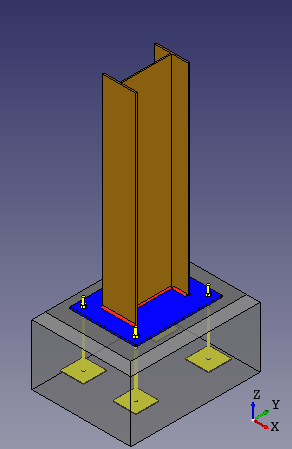
\includegraphics[width=\linewidth]{E:/office _anjali/columnspliceanjali/Osdag3/ResourceFiles/images/3d.png}%
\caption{3D View}%
\end{figure}

%
\end{document}